\chapter{Analyse des besoins}

\section{Fonctionnement de l'application}

Nous posons d'abord les bases de l'application, c'est à dire son foctionnement global, tous les états dans lesquels il sera possible de se trouver, comment y arriver et comment en sortir.

 \begin{figure}[!ht]
 \begin{center}
  \fbox{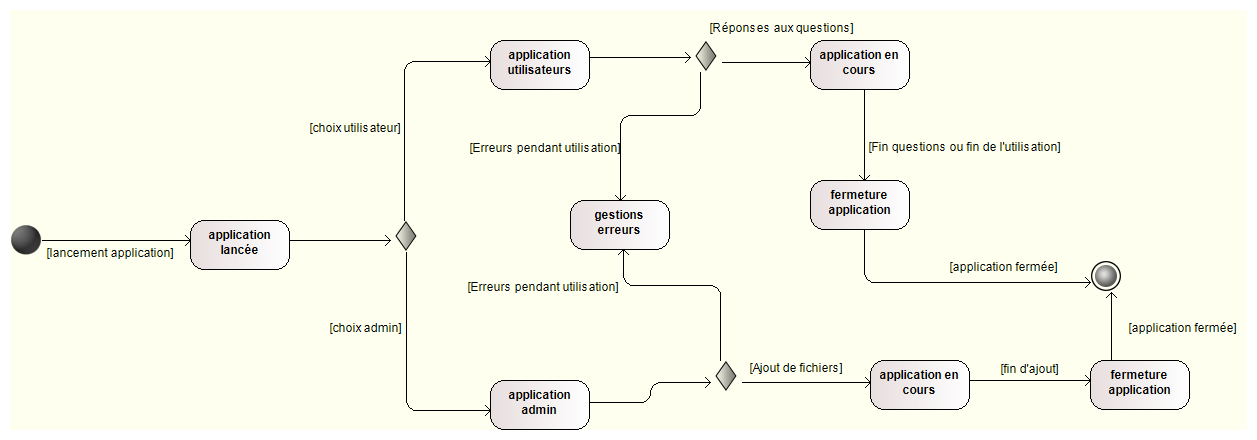
\includegraphics[width=17cm]{besoins/etattrans.png}}
  \caption{Diagramme d'états - Fonctionnement de l'application}
  \label{etattrans}
 \end{center}
 \end{figure}


 La \textsc{Figure} \ref{etattrans} décrit le fonctionnement de l'application, \textit{i.e.} les différents états dans lesquels il est possible de se trouver durant l'utilisation de l'application.


 \begin{figure}[!ht]
 \begin{center}
  \fbox{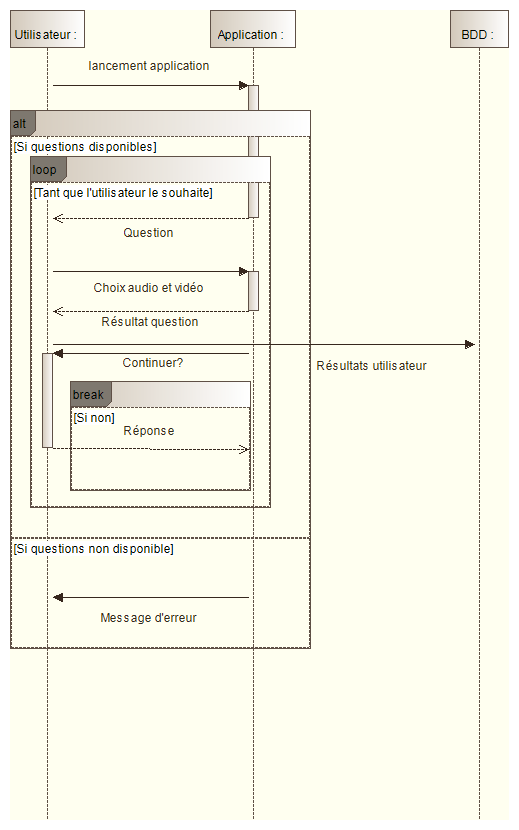
\includegraphics[width=8cm]{besoins/sequence.png}}
  \caption{Diagramme de séquences - Fonctionnement de l’application utilisateur mode Questions/Réponses}
  \label{sequence}
 \end{center}
 \end{figure}

 La \textsc{Figure} \ref{sequence} est en rapport avec le diagramme précédent (\textsc{Figure} \ref{etattrans}). Il décrit les relations entre les différents états de transition.

\section{Classement par priorité des besoins}\label{priorite}

Les besoins sont classés par priorité dans leur ordre d'apparition. De plus, chaque besoin se voit attribué un niveau de priorité comme suit :

\begin{itemize}
 \item[-] Priorité critique
 \item[-] Priorité moyenne
 \item[-] Priorité basse
 \item[-] Facultatif
\end{itemize}

\section{Besoins fonctionnels}\label{besoins_fonctionnels}

\subsection{Utiliser l’application sur les systèmes d’exploitation principaux et récents}\label{systems}

\subsubsection{Description}

Etant donné que notre client sera amené à transporter l’application, il faut que celle-ci puisse fonctionner sur différents environnements à savoir \textit{Microsoft Windows 7}, \textit{Ubuntu 12.04}, \textit{Debian 6.0}, \textit{MAC OS X 10.9} et les versions plus récentes de ces systèmes d’exploitation.
L’application est susceptible de fonctionner sur d’autres systèmes d’exploitation (par compatibilité de noyau) sans toutefois de garantie de ce fonctionnement.

\subsubsection{Faisabilité}

Cette condition est remplie en utilisant une application \textit{JavaFX}, supportée par les environnements possédant un environnement \textit{Java} à jour (la version 8 étant nécessaire pour le fonctionnement optimal de \textit{JavaFX}).

\subsubsection{Contingence}

Le risque principal serait que le client travaille sur une machine ne possédant pas un environnement \textit{Java} à jour. Pour pallier à ce problème, nous avons proposerons un script d'installation du dernier environnement \textit{Java}.

\subsubsection{Test}

Lancer l'application dans chacun des systèmes d’exploitation cités précédemment. L'application devra fonctionner sur chacun de ces systèmes d'exploitation, sans quoi, la contrainte ne serait pas remplie.

\subsubsection{Priorité : \textit{Critique}}

\subsection{Rendre l'application nomade}\label{nomadite}

\subsubsection{Description}

Pour effectuer ses études, notre client ne souhaite pas transporter sa machine sur les lieux où elles se déroulent. Pour cela, il faut donc avoir une application transportable sur un périphérique externe de type clef USB.

\subsubsection{Faisabilité}

Pour remplir cette condition, tous les composants de l’application compilée seront stockés sur une clef USB ou un disque dur externe, afin que le client puisse l'utiliser sur n’importe quel ordinateur.

\subsubsection{Contingence}

Le risque serait que le formatage de la partition de la clef USB ne soit pas pris en compte par le système d’exploitation de la machine (par exemple le formatage \textit{NTFS} de \textit{Windows} est reconnu par le système \textit{Mac OS}, mais accessible en lecture seule, le formatage \textit{EXT4} du système \textit{Ubuntu} n’est pas reconnu par les systèmes d’exploitation \textit{Windows}). Pour éviter cela, la clef devra être formatée en \textit{FAT32}, qui est un formatage de partition reconnu par les systèmes d’exploitation cités dans la section \ref{systems}.

\subsubsection{Test}

Faire fonctionner l’application à partir d’une clef USB (ou disque dur externe selon le support qui sera choisi) sur les différents systèmes d’exploitations cités précédemment. L'application devra fonctionner en \textit{standalone}, sauf dans le cas d'un environnement \textit{Java} non à jour, comme précisé en \ref{systems}.

\subsubsection{Priorité : \textit{Critique}}

\subsection{Ajouter du contenu multimédia et des questions}

\subsubsection{Description}

Le client doit pouvoir enregistrer dans la base de données, de nouvelles vidéos et de nouveaux sons afin d’augmenter l’efficience de ses tests. De plus, pour améliorer ses recherches, notre client pourra ajouter des questions avec leurs correspondances audios et vidéos.
Cet ajout de médias devra être possible en ligne de commande sous un système \textit{Unix}, en passant un fichier texte dans un paramètre.

\subsubsection{Faisabilité}

Pour faciliter cette gestion, nous utiliserons une base de données. Les données seront plus facilement accessibles lors de l’utilisation de l’application.
Puis, pour réaliser l'administration en ligne de commande, une application annexe sera développée. Cette application sera en \textit{Java} et disposera des arguments nécessaires pour ajouter et lister les médias dans la base de données.

\subsubsection{Test}

Ajouter du contenu multimédia (audio et video) et une question puis lister tout le contenu de la base de données pour voir si l’ajout à été pris en compte.
Une réussie du test se concluera par une base de données remplie via l'application annexe, et une application graphique qui fonctionnera (qui accèdera au médias et les affichera).

\subsubsection{Priorité : \textit{Moyenne}}

\subsection{Exploiter différents formats de fichiers audio et vidéo}

\subsubsection{Description}

Le contenu multimédia de notre client étant composé de différents formats vidéos et audios, utilisants des codecs variés, l’application doit pouvoir assurer une lecture optimale de ces médias.

Effectivement, c’est un obstacle que l’on rencontre dès que l’on commence à programmer dans le domaine de la vidéo et de l’audio (des références étudiant certaines de ces contraintes : \cite{ghanbari1999video} et \cite{he2013introduction}).
Le fond du problème est l’utilisation de Codecs (vidéo et audio) pour lire les différents types de fichiers, qui sont encodés selon différentes normes.

Les formats que l’on doit pouvoir supporter sont les suivants :\\

%\begin{table} Fait planter le positionnement vertical du tableau.
\begin{center}
\begin{tabular}{c|c}
\textbf{Formats audio} & \textbf{Formats vidéo} \\
\\
\hline
\\
\textit{mpeg2} & \textit{mp4 (H.264)}\\
\textit{aac} & \textit{mov}\\
\textit{wav} & ~
\end{tabular}
\end{center}
%\end{table}
\vspace{0.6cm}

\subsubsection{Faisabilité}

Une solution que nous avons trouvé est le lecteur de médias \textit{VLC Media Player} \cite{solutions2006vlc}.

Ce lecteur va nous permettre d'utiliser les formats vidéo et audio présentés précédemment. De plus, c'est un logiciel accessible (gratuit et sous licence open-source).

De surcroit, il existe une version portable de \textit{VLC Media Player} permettant un transport optimal sur une clef USB ou un disque dur externe. Cette condition répond à notre besoin de transportabilité évoqué précédemment.

\subsubsection{Contingence}

%Partie a modifier pour le jvlc
Le risque d’utiliser ce genre de logiciel peut être l'impossibilité d'intégrer le lecteur dans une interface graphique \textit{JavaFX} (solution choisie dans la section \ref{systems}). Si cette solution n’est pas possible, on pourra ouvrir un lecteur en \textit{standalone}\footnote{Utilisation de l'application à part entière, et pas dans un plugin ou une extension.}.

\subsubsection{Test}

Création d’un script qui ouvrira toutes les vidéos disponibles et vérifiera si une erreur est survenue.

\subsubsection{Priorité : \textit{Moyenne}}

\subsection{Récupérer les questions et résultats des tests}

\subsubsection{Description}

L’application a pour but de répondre à une série de questions dont les réponses sont une vidéo et un son.\\
Ces combinaisons sont importantes pour notre client, nous devons donc les récupérer.

\subsubsection{Faisabilité}

La solution à ce besoin serait une base de données, stockant l’ensemble des questions, sons, vidéos et réponses attendues.
L’application devra ensuite exporter les réponses et l'identité de l'utilisateur sous forme d’un fichier \textit{txt}, fichier qu’exploitera le client.   

\subsubsection{Test}

Faire faire le test à un faux sujet, et vérifier les données exportées dans le fichier \textit{txt}. Il sera possible de lire le contenu de cet export facilement, avec un éditeur de texte.

\subsubsection{Priorité : \textit{Moyenne}}

\subsection{Rassembler des informations sur les sujets}

\subsubsection{Description}

Afin de pouvoir exploiter les résultats des tests, le client veut récupérer des informations sur les sujets.
Les informations que l’on doit récupérer sont les suivantes :\\
\begin{itemize}
 \item[-]  nom
 \item[-]  prénom
 \item[-]  sexe
 \item[-]  date de naissance
 \item[-]  langue maternelle
 \item[-]  si la langue maternelle est différente de celle du test, nombre d’année d’études de cette langue
\end{itemize}

\subsubsection{Faisabilité}
  
Pour répondre à ce besoin, il faut implémenter un formulaire au lancement de l’application.

\subsubsection{Test}

Faire essayer l’application à une personne tierce, puis, vérifier que toutes les informations sur la personne ont bien été récupérées.

\subsubsection{Priorité : \textit{Faible}}

\section{Besoins non-fonctionnels}\label{besoins_non-fonctionnels}

\subsection{Permettre une maintenance du logiciel}

\subsubsection{Description}

L’application que nous allons livrer ne sera pas une finalité mais seulement une étape dans un projet beaucoup plus vaste. Ainsi, d’autres personnes devront probablement modifier cette application afin de répondre à de nouveaux besoins. Ces nouveaux développeurs devront disposer de tous les éléments nécessaires pour comprendre notre travail. 

\subsubsection{Faisabilité}

Il est possible de répondre à ce besoin en documentant notre code. Il existe par exemple en \textit{Java}, la \textit{Javadoc}, qui est générable avec des commentaires spéciaux. Elle est exportable en \textit{HTML} et contient toutes les explications necessaires à la compréhension du code. 

De plus, il faudra ajouter des commentaires quand une fonction sera trop complexe et que des indications intermédiaires seront nécessaires.

\subsubsection{Test}

Demander à un développeur externe au projet d’essayer de comprendre notre code, et d'ajouter une fonctionnalité.

\subsubsection{Priorité : \textit{moyenne}}

\subsection{Bénéficier d’une ergonomie efficiente}

\subsubsection{Description}

L’application sera ergonomique pour permettre au sujet de se concentrer un maximum sur le test et pas sur le fonctionnement de ladite application. De plus, le sujet soumis au test sera possiblement novice en informatique, l’application devra ainsi être intuitive.

\subsubsection{Faisabilité}

Pour satisfaire ce besoin, nous devons mettre en place un graphisme épuré de tout accessoires détournant l’attention. De plus, nous utiliserons des couleurs de ton pastel pour éviter de fatiguer le regard de l’utilisateur.

Cette contrainte est satisfaisable en s’inspirant de nombreux designs qui ont déjà été développés et publiés sur le web. On s’appuiera notamment sur l’article \cite{lente2014scenariser} qui étudie la \textit{“collaboration entre Ergonomie, Design et Ingénierie”}.

\subsubsection{Test}

Utilisation de l’application par plusieurs sujets sans donner d’indication sur son fonctionnement afin d’observer si le design affecte négativement l'expérience de l’utilisateur.

\subsubsection{Priorité : \textit{basse}}

\section{Prototype d'application}

 En annexe, un \textbf{\textit{prototype}} de l'application que nous avons développé est présenté. Le rendu final que nous présentons diffère quelques peu de ce prototype.

\section{Gestion du temps}

Nous avons établi un calendrier de projet qui présente le déroulement général du projet.

\begin{figure}[!ht]
 \begin{center}
   \fbox{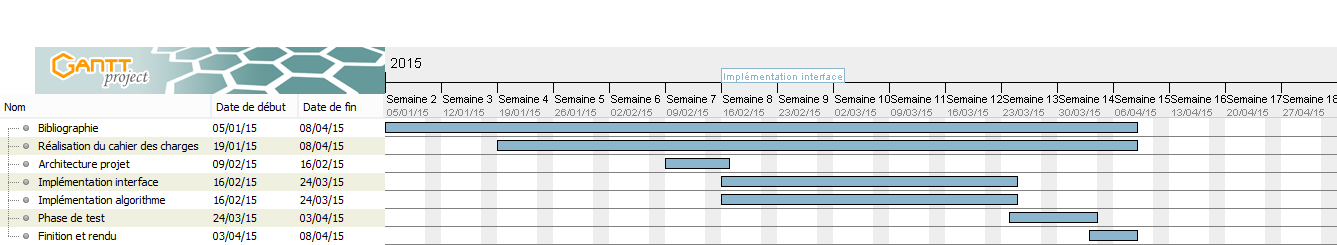
\includegraphics[width=18cm,angle=90]{besoins/gantt.png}}
   \caption{\label{gantt} Gantt - Calendrier du projet}
 \end{center}  
\end{figure}
